\section{Auswertung}
\label{sec:Auswertung}
\subsection{Messdaten}
\label{sec:mess}
Im Folgenden sind die bei der Messung aufgenommenen Daten tabellarisch dargestellt.
\begin{table}[H]
    \centering
    \caption{Der Anodenstrom $I_A$ für verschiedene Anodenspannungen $U_A$ und Heizströme $I_H$.}
    \label{tab:mess1}
    \sisetup{table-format=1.2}
    \begin{tabular}{S[table-format=3.0] S S S S S}
        \toprule
        &
        \multicolumn{5}{c}{$I_A [\si{\milli\ampere}]$}\\
        \cmidrule(lr){2-6}
        {$V_A [\si{\volt}]$} &
        {$I_H=\SI{2.1}{\ampere}$} & {$I_H=\SI{2.2}{\ampere}$} & {$I_H=\SI{2.3}{\ampere}$} & {$I_H=\SI{2.4}{\ampere}$} & {$I_H=\SI{2.5}{\ampere}$} \\
        \midrule
        0    &  0.00  &  0.00  &  0.00  &  0.00  &  0.00 \\
        10   &  0.02  &  0.02  &  0.02  &  0.03  &  0.03 \\
        20   &  0.05  &  0.06  &  0.06  &  0.08  &  0.07 \\
        30   &  0.09  &  0.11  &  0.12  &  0.14  &  0.14 \\
        40   &  0.13  &  0.16  &  0.18  &  0.21  &  0.21 \\
        50   &  0.16  &  0.22  &  0.26  &  0.29  &  0.30 \\
        60   &  0.19  &  0.28  &  0.34  &  0.37  &  0.40 \\
        100  &  0.25  &  0.50  &  0.65  &  0.79  &  0.83 \\
        125  &  0.26  &  0.57  &  0.85  &  1.06  &  1.17 \\
        150  &  0.27  &  0.61  &  0.98  &  1.36  &  1.56 \\
        175  &  0.27  &  0.63  &  1.07  &  1.58  &  1.88 \\
        200  &  0.28  &  0.64  &  1.12  &  1.80  &  2.21 \\
        225  &  0.28  &  0.65  &  1.16  &  1.99  &  2.55 \\
        250  &  0.28  &  0.65  &  1.18  &  2.15  &  2.86 \\
        \bottomrule
    \end{tabular}
\end{table}
\begin{table}[H]
    \centering
    \caption{Die Heizspannung $U_H$ für verschiedene Heizströme $I_H$.}
    \label{tab:mess2}
    \sisetup{table-format=1.1}
    \begin{tabular}{S S}
      \toprule
      {$I_H [\si{\ampere}]$} & {$U_H [\si{\volt}]$}\\
      \midrule
      2.1 & 4.0 \\
      2.2 & 4.1 \\
      2.3 & 4.9 \\
      2.4 & 5.0 \\
      2.5 & 5.5 \\
      \bottomrule
    \end{tabular}
\end{table}
\begin{table}[H]
  \centering
    \caption{Die Anodenstromstärke $I_A$ für niedrige Anodenspannungen $U_A$ bei $I_A=\SI{2.5}{\ampere}$.}
    \label{tab:mess3}
    \sisetup{table-format=3.1}
    \begin{tabular}{S[table-format=1.2] S}
      \toprule
      {$U_A [\si{\volt}]$} & {$ I_A [\si{\nano\ampere}]$}\\
      \midrule
      0.0  &   14.5 \\
      0.1  &   23.6 \\
      0.2  &   33.0 \\
      0.3  &   51.0 \\
      0.4  &   75.0 \\
      0.5  &   90.0 \\
      0.6  &  130.0 \\
      0.7  &  171.0 \\
      0.8  &  216.0 \\
      0.9  &  268.0 \\
      0.96 &  300.0 \\
      \bottomrule
    \end{tabular}
\end{table}

\subsection{Kennlinien}
\label{sec:kenn}
Die Daten aus Tabelle \ref{tab:mess1} sind in Abbildung \ref{fig:plot1} graphisch dargestellt. Um die Lesbarkeit zu erhöhen, wurden die Messdaten
farbig verbunden.
\begin{figure}[H]
    \centering
    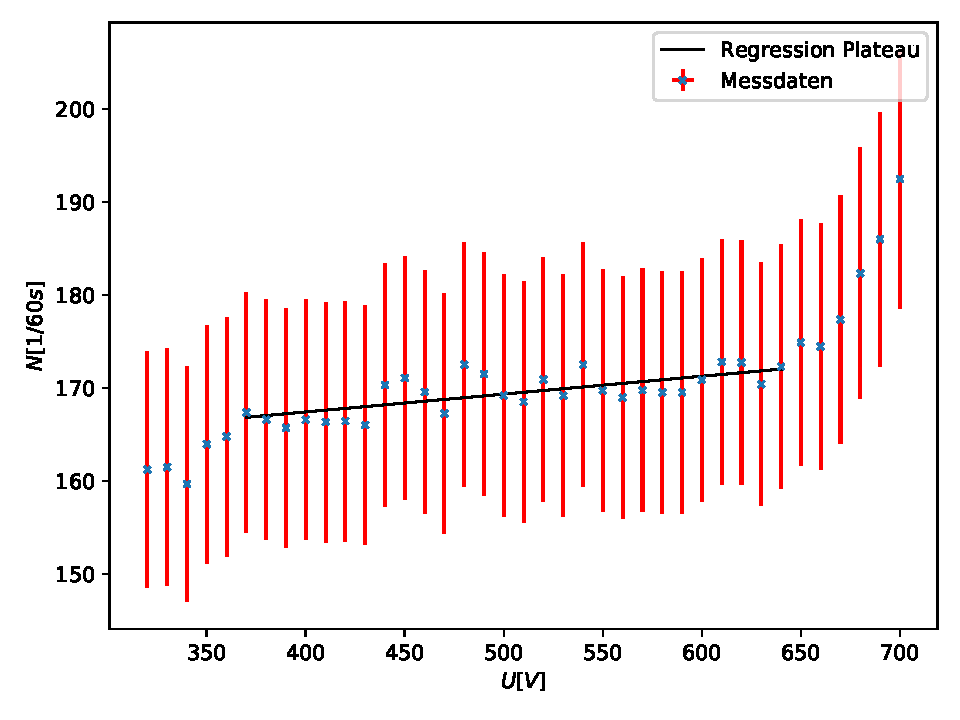
\includegraphics[scale= 0.8]{auswertung/plot1.pdf}
    \caption{Die Kennlinien für verschiedene Heizströme.}
    \label{fig:plot1}
\end{figure}
\noindent
Die aus der Abbildung abgeschätzten Sättigungsströme $I_S$ sind in Tabelle \ref{tab:satt} aufgelistet. Da für die Heizströme $I_A=\SI{2.4}{\ampere}$
und $I_A=\SI{2.5}{\ampere}$ der Sättigungsstrom nicht direkt abgelesen werden kann, wurde der Wendepunkt der Kennlinie geschätzt und die dabei
abgelesene Stromstärke verdoppelt. Die geschätzten Wendepunkte sind dabei $(\SI{125}{\volt}, \SI{1.06}{\milli\ampere})$ für $I_A=\SI{2.4}{\ampere}$
und $(\SI{150}{\volt}, \SI{1.56}{\milli\ampere})$ für $I_A=\SI{2.5}{\ampere}$.
\begin{table}[H]
    \centering
      \caption{Die Sättigungsströme für verschiedene Heizströme.}
      \label{tab:satt}
      \sisetup{table-format=1.2}
      \begin{tabular}{S[table-format=1.1] S}
        \toprule
        {$I_H [\si{\ampere}]$} & {$ I_S [\si{\milli\ampere}]$}\\
        \midrule
        2.1 & 0.28 \\
        2.2 & 0.65 \\
        2.3 & 1.18 \\
        2.4 & 2.12 \\
        2.5 & 3.12 \\
        \bottomrule
    \end{tabular}
\end{table}

\subsection{Der Exponent des Langmuir-Schottkyschen Gesetzes}
\label{sec:langschott}
Der Geltungsbereich des Langmuir-Schottkyschen Gesetzes reicht von dem Ursprung bis zu dem Wendepunkt der Kennlinie. Für den maximalen Heizstrom
von $I_H=\SI{2.5}{\ampere}$ kann das Intervall demnach auf $[\SI{0}{\volt}, \SI{150}{\volt}]$ geschätzt werden. In Abbildung \ref{fig:plot2} sind
die Messwerte in diesem Intervall in log-log-Darstellung aufgetragen.
\begin{figure}[H]
    \centering
    \includegraphics[scale= 0.8]{auswertung/plot2-2.pdf}
    \caption{Die Kennlinien für $I_A=\SI{2.5}{\ampere}$ im Intervall $[\SI{0}{\volt}, \SI{150}{\volt}]$ in doppellogarithmischer Darstellung.}
    \label{fig:plot2}
\end{figure}
\noindent
Das Langmuir-Schottkysche Gesetz ist durch die logarithmischen Darstellung in der Form
\begin{align*}
    \log(I/\si{\ampere})&=a\cdot \log(U\si{\volt})+b\\
    \Leftrightarrow
    (I/A)&=\text{e}^b(U/V)^{a},  %großes Uff bei den Einheiten
\end{align*}
sodass die eingezeichnete Regression der Form
\begin{equation}
    y=m\cdot x+b
    \label{eqn:gerade}
\end{equation}
ist. Die Regression wurde von \textit{numpy} \cite{numpy} mit den Parametern
\begin{align*}
    a &= \SI{1.48   \pm 0.020}{} \\
    b &= \SI{-13.90 \pm 0.080}{} 
\end{align*}
berechnet. Der gefragte Exponent des Langmuir-Schottkyschen Gesetzes ist gerade der Parameter $a$. Verglichen mit dem Theoriewert von $3/2$
ergibt sich eine prozentuale Abweichung von $p=\num{1.35}\%$

\subsection{Anlaufstromgebiet}
\label{sec:anlauf}
Die Messwerte der Anodenspannung und Stromstärke für die maximale Heizleistung von $I_H=\SI{2.5}{\ampere}$ sind in Tabelle \ref{tab:mess3}
aufgelistet. Da für die Messung ein Amperemeter mit einem Innenwiderstand von $R_i=\SI{1}{\mega\ohm}$ verwendet wurde, muss die Spannung
zu 
\begin{equation*}
    U_k=U+I\cdot R_i
\end{equation*}
korrigiert werden. In Abbildung \ref{fig:plot3} sind die Daten in einer log-lin-Darstellung abgebildet. 
\begin{figure}[H]
    \centering
    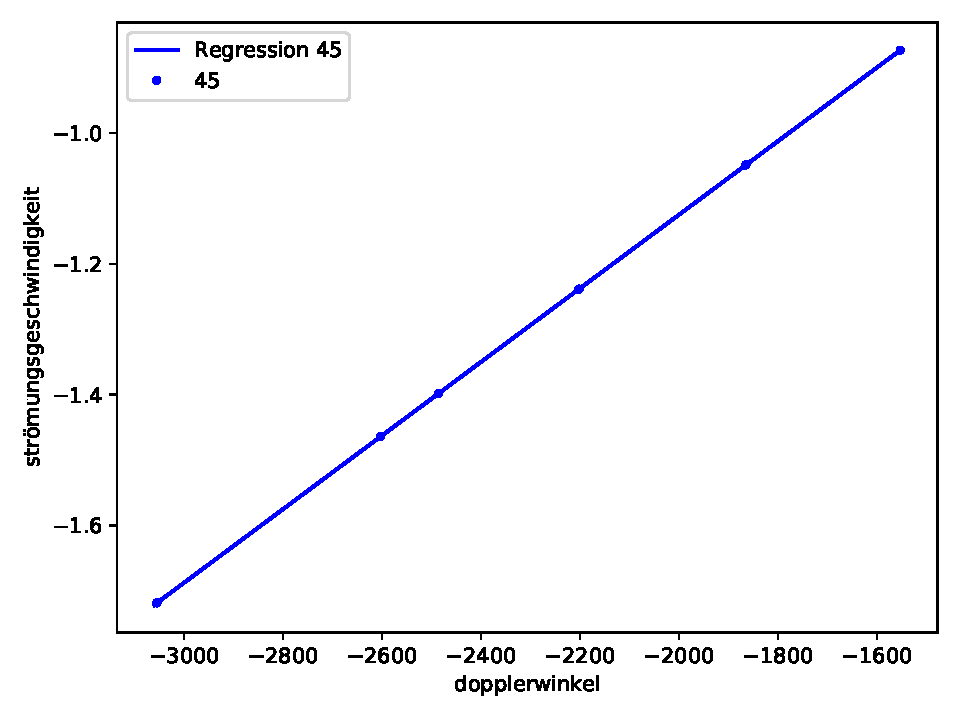
\includegraphics[scale= 0.8]{auswertung/plot3.pdf}
    \caption{Kennlinie für $I_H=2.5$ im Anlaufstrmgebiet.}
    \label{fig:plot3}
\end{figure}
\noindent
Die von \textit{scipy} \cite{scipy} berechnete Regression ist somit wieder linear, also der Form von Gleichung \eqref{eqn:gerade} mit den Parametern
\begin{align*}
    a &= \SI{  3.11 \pm 0.127}{\per\volt}\\
    b &= \SI{-38.56 \pm 0.074}{}    .
\end{align*}
Die Gerade entspricht dabei dem Logarithmus der Gleichung \eqref{eqn:anlaufstrom}.
Mit der Steigung $a$ der Geraden lässt sich nun mittels
\begin{equation*}
    T=\frac{\symup{e_0}V}{ka}
\end{equation*}
die Kathodentemperatur bestimmen. Durch Einsetzen ergibt sich
\begin{equation*}
    T=\SI{3736.62 \pm 152.79}{\kelvin}  .
\end{equation*}
Die Unsicherheit wurde dabei von \textit{uncertainties} \cite{uncertainties} berechnet.

\subsection{Berechnung der Kathodentemperatur mittels Heizleistung}
\label{sec:temp}
Die Katohdentemperatur kann auch mit der Heizleistung durch Ausnutzen von Gleichung \eqref{eqn:heizleistung} berechnet werden. Das Umstellen
der Gleichung \eqref{eqn:heizleistung} liefert
\begin{equation*}
    T=\sqrt[4]{\frac{I_H U_H-N_{WL}}{f\eta\sigma}}
\end{equation*}
mit den Konstanten
\begin{align*}
    N_{WL} &= \SI{0.95      }{\watt} \\
    f      &= \SI{0.32 e-4}{\square\metre}\\
    \sigma &= \SI{5.7  e-8}{\watt\per\square\metre\per\kelvin\tothe{4}}\\
    \eta   &= \num{0.28      }  .
\end{align*}
<<<<<<< HEAD
Die Kathodentemperaturen in Tabelle \ref{tab:T} werden durch Einsetzten der Messdaten für die Heizleistung aus Tabelle \ref{tab:mess2}
berechnet. 
\begin{table}[H]
    \centering
      \caption{Die berechnete Katohdentemperatur für verschiedene Heizleistungen.}
      \label{tab:T}
      \sisetup{table-format=4.2}
      \begin{tabular}{S[table-format=1.1] S[table-format=1.2] S}
        \toprule
        {$I_H [\si{\ampere}]$} & {$ U_H [\si{\volt}]$} & {$T [\si{\kelvin}]$}\\
        \midrule
        2.1 & 4.0 & 1954.31 \\
        2.2 & 4.1 & 1993.76 \\
        2.3 & 4.9 & 2120.19 \\
        2.4 & 5.0 & 2156.73 \\
        2.5 & 5.5 & 2237.47 \\
        \bottomrule
    \end{tabular}
\end{table}

\subsection{Austrittsarbeit}
\label{sec:phi}
Mit der Richardson-Gleichung \eqref{eqn:richardson} kann nun die Austrittsarbeit $\Phi_W$ von Wolfram bestimmt werden, indem diese zu 
\begin{equation*}
    \Phi=\frac{-kT}{\symup{e_0}}\log{\left(\frac{I_Sh^3}{4\pi\symup{e_0}m_0fk^2T^2}\right)}
\end{equation*}
umgestellt wird. Dabei sind $I_S$ die geschätzten Sättigungsströme aus Tabelle \ref{tab:satt} $T$ die berechneten Kathodentemperaturen
aus Tabelle \ref{tab:T}. Die somit berechnete Austrittsarbeit $\Phi_W$ wurde für alle fünf Heizleistungen berechnet. Dann wurde von
\textit{numpy} \cite{numpy} der Mittelwert, sowie die Unsicherheit berechnet
\begin{equation*}
    \Phi_W=\SI{5.26 \pm 0.07}{\electronvolt}    .
\end{equation*}
Die prozentuale Abweichung zu dem Literaturwert $\Phi_{lit}=\SI{4.54}{\electronvolt}$ \cite{AP02} beträgt $p=\num{15.9}\%$.
